\question 结构(Cobegin语句1;语句2 Coend)表示语句1和语句2并发执行。程序段如下:

~
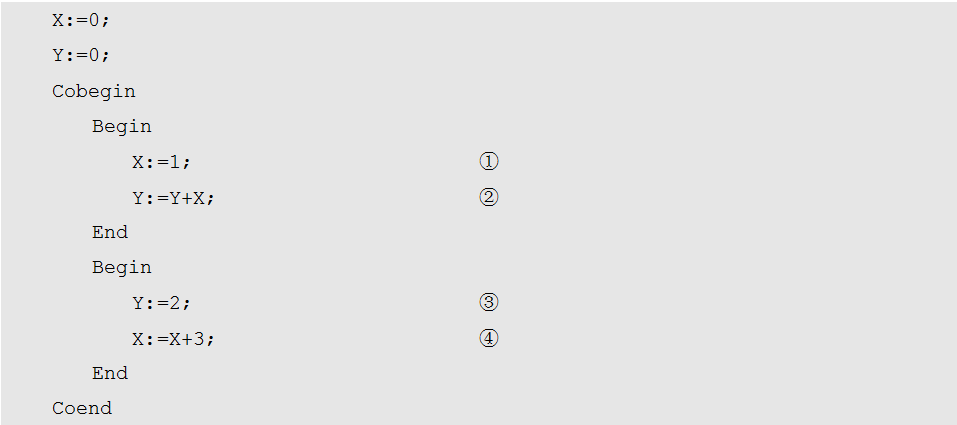
\includegraphics[width=2.42708in,height=1.07292in]{computerassets/4DDE49E225C2295AEB3F23EAC5BBDEF5.png}

当这个程序执行完时,变量X和Y的值有可能为( ~)。 Ⅰ.X=1,Y=2 Ⅱ.X=1,Y=3
Ⅲ.X=4,Y=6
\par\twoch{Ⅰ}{Ⅰ和Ⅱ}{\textcolor{red}{Ⅱ和Ⅲ}}{Ⅰ、Ⅱ和Ⅲ}
\begin{solution}由于语句并发执行,因此可能的执行顺序有①②③④(X=4,Y=2)、①③②④(X=4,Y=3)、①③④②(X=4,Y=6)、③④①②(X=1,Y=3),③①②④(X=4,Y=3)、③①④②(X=4,Y=6)这6种情况。所以应该选C。这类题主要考查对于并发执行的理解,列出所有可能情况时,注意Begin和End中的语句还是按顺序执行的。
\end{solution}
\question (南京航空航天大学,2006年)要实现两个进程互斥,设一个互斥信号量mutex,当mutex为0时,表示
\par\twoch{没有进程进入临界区}{\textcolor{red}{有一个进程进入临界区}}{有一个进程进入临界区,另外一个进程在等候}{两个进程都进入临界区}
\begin{solution}当仅有两个并发进程共享临界资源时,互斥信号量仅能取值1、0、-1,互斥信号量的初始值设为1。即当互斥信号量初值为1时,表示同时只允许1个进程访问临界资源。当有1个进程提出访问临界资源请求时,执行P操作,互斥信号量减1,变为0,同时该进程进入临界区。如果另一个进程此时也请求访问临界资源,则同样执行P操作。由于互斥信号量执行P操作之前的值为0,执行过P操作后,信号量值变为-1。
综上所述,mutex为1时,表示没有进程进入临界区;mutex为0时,表示有一个进程已进入临界区;mutex为-1时,表示有一个进程进入临界区,另一个进程等待进入。
\end{solution}
\question 在9个生产者、6个消费者共享容量为8的缓冲器的生产者---消费者问题中,保证进程互斥使用缓冲器的信号量初值为
\par\twoch{\textcolor{red}{1}}{6}{8}{9}
\begin{solution}用来控制互斥的信号量初值应当等于允许的同时最大访问进程数,缓冲器同时只允许一个进程使用,因此互斥信号量的初值为1。不要被题目中给的其他条件混淆。
\end{solution}
\question 进行p0和p1的共享变量定义及其初值为: boolean flag{[}2{]}; int turn=0;
flag{[}0{]}=FALSE; flag{[}1{]}=FALSE;
若进行p0和p1访问临界资源的类C代码实现如下: void p0() //进程p0 \{ while
(TRUE) \{ flag{[}0{]}=TRUE; turn=1; While (flag{[}1{]}\&\&(turn==1));
临界区; flag{[}0{]}=FALSE; \} \} void p1() //进程p1 \{ while (TRUE) \{
flag{[}1{]}=TRUE; turn=0; While (flag{[}0{]}\&\&(turn==0)); 临界区;
flag{[}1{]}=FALSE; \} \} 则并发执行进程p0和p1时产生的情形是( )
\par\fourch{不能保证进程互斥进入临界区,会出现“饥饿”现象}{不能保证进程互斥进入临界区,不会出现“饥饿”现象}{能保证进程互斥进入临界区,会出现“饥饿”现象}{\textcolor{red}{能保证进程互斥进入临界区,不会出现“饥饿”现象}}
\begin{solution}在之前没有了解过该算法的情况下,临场想要判断出来还是比较困难的,尤其本题的算法是一个可以保证进程互斥进入临界区且不会出现饥饿现象的良好算法,在考虑的时候,没法找出破绽,还容易误认为自己的想法不够全面而耽误时间。
下面分析算法。
首先是初始化步骤。第一步是初始化两个数组元素为FALSE,表明初始状态两个进程都没有打算进入临界区。第二步是turn置为0,这里的turn置为0并没有特殊的用意,有些读者会理解为优先执行进程P0,其实仔细分析并不是。因为对于turn的赋值操作都是在对turn的判断之前,也就是在程序执行开始后,都会先对turn值进行操作,然后才会判断,这里turn=0的用意仅仅是对turn值进行一个初始化,改为turn=1的效果也是完全相同的。
其次分析每个进程的执行流程(本题解释有些烦琐,如果已经掌握本题,跳过即可。对于不熟悉本题的读者,请紧跟解析,一次看完,中途打断思路可能会跟不上)。
由于进程P0和P1的执行流程类似,所以分析进程P0即可。假设此时进程P0要访问临界资源,进程P1尚未执行,开始执行题目中的代码,首先会进入第一个while循环(while(TRUE)),循环中第一行语句为``flag{[}0{]}=TRUE;
turn=1;'',将代表自己的flag置为TRUE,并将turn置为1,表明进程P0要申请访问临界资源(flag{[}0{]}=TRUE),并表明自己访问结束之后轮到进程P1访问临界资源(turn=1)。
接下来语句为``While
(flag{[}1{]}\&\&(turn==1));''。这句是很多考生粗心看错且很难弄明白含义的一个语句,本语句有着保证避免饥饿现象和互斥访问的作用,为本题的关键所在。
首先要注意这个while循环语句的最后有一个分号,表明该语句的含义是如果满足条件则执行空语句,直到不满足条件才跳出循环执行下面的语句,即不满足条件才进入临界区。在这一点上很多考生粗心漏看了分号而误认为本句是满足条件才进入临界区。
然后分析这句为什么能保证互斥访问和避免饥饿现象。先解释为什么能保证互斥。如果进程P1正在访问临界区,则相关变量的值为flag{[}0{]}=FALSE,flag{[}1{]}=TRUE,turn=0,这时候如果进程P0请求访问临界区,则会将flag{[}0{]}赋值为TRUE,turn赋值为1,此时相关变量就变为flag{[}0{]}=TRUE,flag{[}1{]}=TRUE,turn=1,此时进程P0会由于满足while循环的条件(flag{[}1{]}\&\&(turn==1))而不断执行空语句,直到进程P1访问完临界资源并将flag{[}1{]}置为FALSE,才能够跳出循环并进入临界区。对于进程P1情况类似,因此该算法能够保证两个进程互斥进入临界区。
接下来解释为什么能够避免饥饿现象。所谓饥饿现象是指某进程请求执行却长期得不到调度。本题中的一种饥饿现象就是进程P1提出申请,但系统却一直执行进程P0,导致进程P1长期得不到调度。分析相关变量情况。当进程P0正在临界区执行,此时进程P1提出进入临界区的请求时,执行``flag{[}1{]}=TRUE;
turn=0;''语句后,相关变量情况为flag{[}0{]}=TRUE,flag{[}1{]}=TRUE,turn=0。等待进程P0本次临界区执行结束(执行了flag{[}0{]}=FALSE;),紧接着进程P0又提出了访问请求,假设处理器总是优先执行进程P0的请求,则进程P0可以无阻碍地执行完``flag{[}0{]}=TRUE;
turn=1;'',此时相关变量情况为flag{[}0{]}=TRUE,flag{[}1{]}=TRUE,turn=1,则此时进程P0会执行语句``While
(flag{[}1{]}
\&\&(turn==1));''。这时候会由于满足条件而不断执行空语句,由于仅仅依靠进程P0已经无法跳出循环(因为此时进程P0已经没有改变,flag{[}1{]}和turn的语句可以执行),这时进程P1也是执行对应的一条语句``While
(flag{[}0{]}\&\&(turn==0));'',由于turn=1,所以进程P1会跳出这个循环并进入临界区执行,因此在假设处理器非常偏心进程P0的情况下进程P1还是会得到执行。进程P1执行完之后,也会有类似情况而使进程P0得到调度执行,所以进程P0和进程P1是交替执行的,本算法并不存在饥饿现象。
实际上,该算法为Peterson算法,满足互斥、空闲让进、有限等待3条同步机制准则,可以达到比较好的同步效果。本算法通过flag数组保证两个进程互斥进入临界区,同时通过turn来保证两个进程交替执行,避免了饥饿现象。本算法的缺点是无法设置进程的优先级,比如不能做到在进程P1提出申请后,仍然使进程P0连续执行多次,只能交替执行。但瑕不掩瑜,这仍然是一个能选出正确选项的好算法。
\end{solution}
